% !TeX program = xelatex
\documentclass{ctexart}
\usepackage[table]{xcolor}
\usepackage{template_by_mny}
\usepackage{float} 
\usepackage{listings}
\lstset{basicstyle=\ttfamily, breaklines=true, frame=single}

\title{光谱仪教学实验报告}
\class{物理 32/物理 31}
\name{冯家琦/周方远}
\id{2023011338/2023011263}

\begin{document}
\maketitle

\begin{abstract}
本实验使用EDU-SPEBCT1扩展光谱仪教学套件,完成了绿光波长测量、样品吸收率光谱图等实验。通过实验加深了对光谱仪工作原理的理解,掌握了光谱测量的进阶方法。
\end{abstract}

\section{实验原理}

反射光栅光谱仪是一种用于分析光谱的光学仪器。其基本原理包括:
\begin{figure}[H]
    \centering
    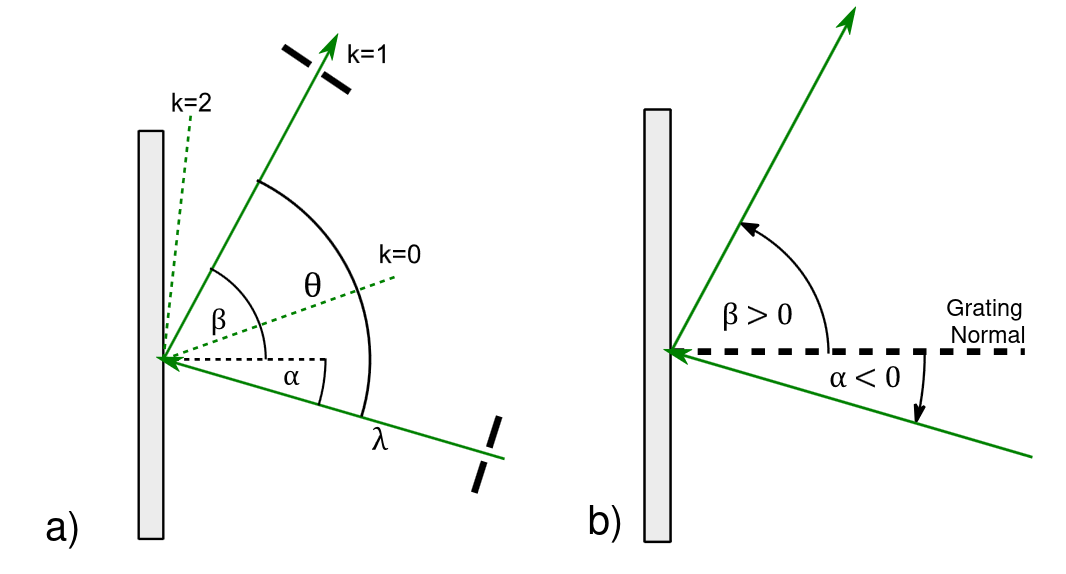
\includegraphics[width=0.6\textwidth,height=0.3\textwidth]{pictures/原理图例.png}
    \caption{衍射角与入射角和级数的关系}
\end{figure}

如图所示,k 表示衍射级数,$\lambda$ 是波长,$\alpha,\beta$ 分别是入射角和出射角,d 为光栅间距。它们满足如下关系:
\[k\cdot\lambda=\sin\beta\cdot d+\sin\alpha\cdot d\]
\subsection{光谱仪的组成}
一个基本的光谱仪包含以下部件:
\begin{itemize}
    \item 入射狭缝:控制入射光束宽度
    \item 反射聚焦镜:将光线聚焦到光栅上
    \item 分光元件:反射光栅
    \item 聚焦系统:再用凹面镜将分光后的光聚焦
    \item 观测屏/探测器:用于观测光谱
\end{itemize}

\section{实验仪器及安装}
\subsection{实验仪器}
\begin{itemize}
    \item EDU-SPEB2光谱仪教学套件
    \item 可调节狭缝
    \item 三棱镜
    \item LED光源及其USB供电支架
    \item 双凸透镜(f=50mm和100mm)
    \item 观测屏
    \item 其他光学元件支架和固定件
\end{itemize}
\subsection{仪器安装}


\section{实验步骤}
\subsection{确定波长}

\subsection{参考光谱}
**

\subsection{样品光谱}
**

\subsection{数据分析:吸收谱线}
**

\section{实验思考}

\section{总结}
**

\end{document}